\lesson{2}{Oct 6 2021 Wen (08:00:23)}{Electromagnetic Radiation}{Unit 2}

At one time, matter and energy were considered distinctly different. Matter had mass and volume; energy did not. Instead, energy traveled in a wave. Comparing the two would be like comparing something physical in your hands to something invisible. At least, that's how it seemed.

\begin{displayquote}
    \textbf{\textit{Electrons behave like waves and particles}}
\end{displayquote}

Then a scientist named \textbf{Max Planck} discovered that energy could have both wavelike and particle-like properties. He also discovered that energy was not continuous, but seemed to transfer in packets. Soon after, Albert Einstein agreed with Planck and added to his hypothesis by proposing that energy transferred in discrete packets called quanta.

Planck's and Einstein's ideas about energy also helped explain the dual nature of electrons. Electrons behave as particles when they orbit in a cloud around the nucleus or when they interact with other substances in a defined position.

To observe electrons behaving as waves, let's look at Feynman's double-slit experiment. In this experiment, a stream of electrons was sent through a wall with two small open slits. The electrons hit the backdrop in specific areas like particles, but when the areas were connected, they showed a wavelike interference pattern. This showed that electrons seemed to have the properties of both particles and waves.

\subsubsection*{characteristics of waves}

Radiation is the emission of energy in the form of waves. All waves are repetitive, come in various sizes, and carry energy. When you think of waves, you may think of waves rolling onto a beach. Although they may move in similar ways, an electromagnetic wave is different from ocean waves because they can travel through the emptiness of space.

The lowest point of a wave is a trough, and the highest point of a wave is a crest. The vertical distance between the crest or trough and the center line of the wave is its amplitude. Amplitude measures the height, or intensity, of the wave.

Here is an image of a wave:

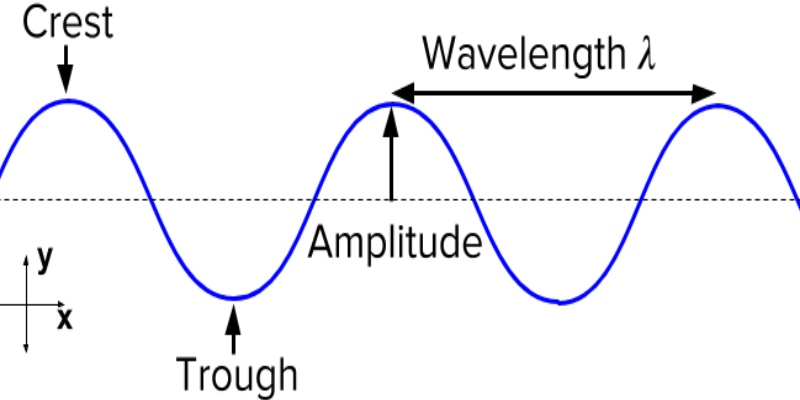
\includegraphics[width=\textwidth,height=\textheight,keepaspectratio]{images/characteristics-of-waves}

\subsubsection*{Electromagnetic Spectrum}

\begin{itemize}
    \item \textbf{Radio Waves}: Radio waves are radiation used for radio, TV antennas, and cell phones.
    \item \textbf{Microwaves}: Microwaves are radiation used in radar and to heat food.
    \item \textbf{Infrared Radiation}: Infrared radiation, also known as infrared light, is heat, which is emitted by all objects. The military uses infrared to see how many people are in buildings or to see people at night.
    \item \textbf{Visible Light}: Visible light is all the radiation humans can see.
    \item \textbf{Ultraviolet}: Ultraviolet light is radiation given off by the sun that causes sunburns.
    \item \textbf{X-rays}: X-rays are radiation used in the medical field to look at people's bones and insides. This type of radiation is created when high-velocity electrons collide.
    \item \textbf{Gamma Rays}: Gamma rays are radiation given off by radioactive substances.
\end{itemize}

\newpage
